\section*{Learning Objectives}

\begin{itemize}
\item Equations with derivatives are called (ordinary) differential equations, or ODEs for short.
\item We model mobile robots with ODEs.
\item Simulation means to solve an ODE numerically with a computer.
\item Balancing is a key problem in robotics.
\end{itemize}

\section*{Outcomes} 
\begin{itemize}
\item Learn about states and controls in ODE models.
\item Learn Euler's method for numerically approximating solutions to ODEs.
\item Apply Euler's method to simulate several simple examples.
\item Learn about the double inverted pendulum.
\item Simulate the double inverted pendulum via Euler's method.
\item For linear models, learn how to compute control sequences that drive the system from an initial state to a desired final state.
\item Feedback means that the values in a control sequence are defined to depend on state of the system.
\item Our main feedback control method involves least squares solutions of underdetermined equations from Chapter 9 or our textbook.
\item Model Predictive Control (MPC) is based on iteratively computing new least squares solutions as the state of the system evolves with time. \url{https://www.youtube.com/watch?v=8U0xiOkDcmw}
\item Balance the double inverted pendulum via MPC.
\end{itemize}

\vspace*{1cm}

\textbf{Either download Lab9 from our Canvas site or open up a Jupyter notebook so that you can enter code as we go. It is suggested that you have line numbering toggled on.}  

\newpage


\section{Motivation}
\begin{itemize}
    \item MS-Degree-level feedback control of the double inverted pendulum on a cart,  \url{https://www.youtube.com/watch?v=B6vr1x6KDaY}. While our work will be simpler than what is shown in this video, we'll still launch you on the path to designing your own feedback control for interesting robot-like devices.
    \item Advanced Undergrad-level feedback control of the double inverted pendulum, \url{https://www.youtube.com/watch?v=W5q_eYd9bfY}. You need at least EECS 460.
    \item A self-balancing stick, another cool feedback control problem: \url{https://www.youtube.com/watch?v=woCdjbsjbPg}. This system depends on controlling angular momentum, something you learn about in Physics 140. 
    \item The feedback control of the Michigan Cassie bipedal robot combines ideas from the above with Differential Geometry, \url{https://www.youtube.com/watch?v=utWqXZwTIbQ}. Differential Geometry is a generalized form of calculus that works on surfaces, such as spheres, and more exotic things, like a Klein Bottle. 
    \item Professor Grizzle started his work on bipedal robots with the simpler robot, Rabbit; see \url{https://www.youtube.com/watch?v=3m-64ZdkuAg} and \url{https://www.youtube.com/watch?v=tHiqlSQsUnA}.
    \item Step by step, pun intended, this led to MABEL running at 3 m/s \url{https://www.youtube.com/watch?v=xlOwk6_xpWo}.
    \item And then Cassie on the Wave Field, \url{https://youtu.be/V36DCsc6iio?t=84}.
    
\end{itemize}


   \begin{figure}[hbt!]%
	\centering
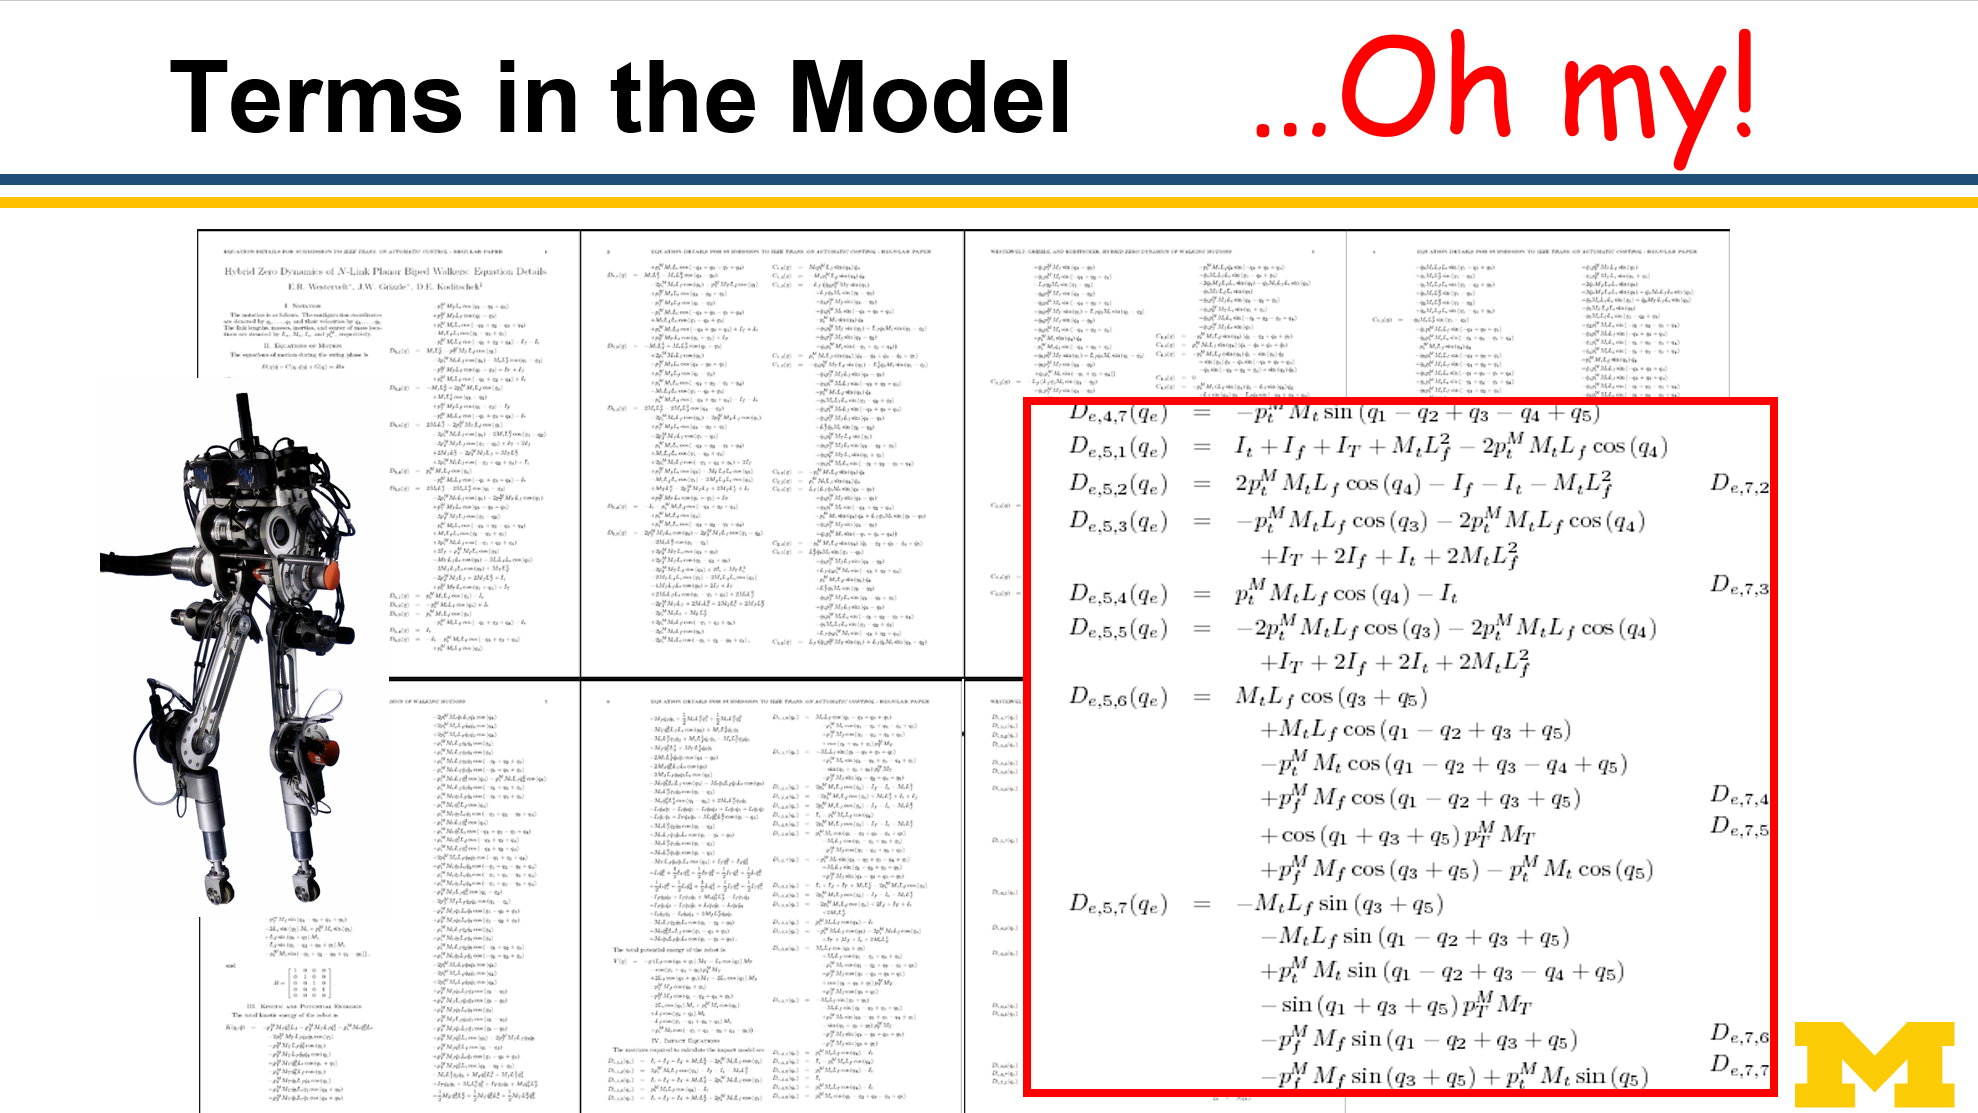
\includegraphics[width=0.99\columnwidth]{graphics/Chap09/RabbitBigModel.png}
    \caption[]{Terms in the ODE that describes (models) the bipedal robot named ``Rabbit'' by its French designers are shown in this figure. A model of the Cassie or Digit bipedal robots is more than 100 times larger. By combining good mathematics and programming skills, Prof. Grizzle's students use these models to design bipedal walking and running gaits; see \url{https://www.youtube.com/user/DynamicLegLocomotion}.}
    \label{fig:RabbitBigModel}
\end{figure}

 \section{What is an ODE?}

Equations with a derivative in them are called \textbf{ordinary differential equations} or \textbf{ODEs for short}. Here is what one may look like,
\begin{equation}
    \label{eq:SampleODE}
    \dot{x}(t) = f(x(t), u(t))
\end{equation}
where $t$ is time, $x(t)$ is a vector of variables that we call ``states'', $\dot{x}(t):=\frac{dx(t)}{dt}$ is the rate of change of $x(t)$ with respect to time, and $u(t)$ is a vector of input variables, such as a motor torque, that we can ``control''. This lab goes all in on ODEs. Why? 
\begin{itemize}
    \item In Robotics, we use differential equations to understand the motion of robots, such as Cassie Blue, or in the case of Project \#3, a Segway.
    \item Because we have studied iterative methods for solving equations, such as the Bisection Method, the Newton-Raphson Algorithm, and Gradient Descent, we are well positioned to approach the solution of differential equations through the lens of iteration. 
    \item  The topic of differential equations is typically delayed until a third- or fourth-semester Calculus course. Such courses focus almost exclusively on closed-form solutions to differential equations, which is a gnarly subject. We, however, will take a numerical approach and thereby allow you to see physics and calculus in a new light. 
    \item The differential equations associated with robot models, such as Rabbit shown in Fig.~\ref{fig:RabbitBigModel}, do not possess closed-form solutions! The equations have solutions, but literally, it has been proven that the solutions cannot be expressed in terms of trigonometric functions, polynomials, ratios, and radicals of such functions.  While closed-form solutions are nice when they exist, as a Roboticist, one has to face reality and deal with the challenges at hand. For more information, see \url{https://en.wikipedia.org/wiki/Three-body_problem#/media/File:Three-body_Problem_Animation_with_COM.gif} and  \url{https://en.wikipedia.org/wiki/Three-body_problem}.
\end{itemize}



In Robotics, we typically deal with ODEs that look like this
\begin{equation}
    \label{eq:EoM_pinned}
    D(q(t))\ddot{q}(t) + C(q(t),\dot{q}(t))\dot{q}(t) + G(q(t)) = Bu(t),
\end{equation}
where 
\begin{itemize}
\item $t$ represents time in seconds,
    \item $q(t)$ is an $n$-vector, consisting of positions and angles,
    \item $\dot{q}(t):= \frac{dq(t)}{dt}$ is the rate of change of $q$,
    \item $\ddot{q}(t):= \frac{d^2q(t)}{dt^2} = \frac{d\dot{q}(t)}{dt}$ is the rate of change of $\dot{q}(t) = \frac{dq(t)}{dt}$,
    \item $D$ is an $n \times n$ matrix whose entries depend on $q$,
    \item $C$ is an $n \times n$ matrix whose entries depend on $q$ and $\dot q$,
    \item $G$ is $n \times 1$ vector whose entries depend on $q$,
    \item $B$ is an $n \times m$ matrix, and 
    \item $u$ is an $m$-vector of controls. 
\end{itemize}
Figure~\ref{fig:RabbitBigModel} shows in very small font some of the terms in the various matrices and vectors for a specific robot. The marriage of math and software allows us to analyze such models for very complicated robots. \\

We can rewrite \eqref{eq:EoM_pinned} in the form \eqref{eq:SampleODE} by defining the state as
$$ x(t) := \begin{bmatrix}  x_1(t) \\ x_2(t)\end{bmatrix} := \begin{bmatrix}  q(t) \\ \dot{q}(t)\end{bmatrix},$$
so that
\begin{equation}
    \label{eq:RobotODE}
    \dot{x}(t) = \left[ \begin{array}{cc} x_2(t) \\
    \left( D(x_1(t))\right)^{-1 } \left( -C(x_1(t),x_2(t))x_2(t) - G(x_1(t))  + Bu(t) \right)
   \end{array}  \right]=: f(x(t), u(t)).
\end{equation}
In later Robotics courses, you will skip the rewriting step and learn how to work directly with \eqref{eq:EoM_pinned} and some of its generalizations!

\section{Euler's Method for Numerically Solving ODEs}

We assume that you have not yet taken any Calculus, and therefore in particular, we assume that you have not yet taken a course on Differential Equations\footnote{At Michigan, that would be Math 216.}. We will emphasize in ROB 101 a very simple numerical method for (approximately) solving differential equations that is due to Euler. You can read more about it in case you are interested:
\begin{itemize}
    \item Wikipedia \url{https://en.wikipedia.org/wiki/Euler_method}
    \item Khan Academy \url{https://www.khanacademy.org/math/ap-calculus-bc/bc-differential-equations-new/bc-7-5/v/eulers-method}
\end{itemize}
The basic idea is based on our forward difference method for computing a derivative of a function. We will assume our function is $x(t)$ and we have an ODE 
\begin{equation}
\boxed{
    \frac{dx(t)}{dt} = f(x(t)),
    }
\end{equation}
where $t$ represents time.\\


To develop a numerical approximation to the ODE, we recall that 
\begin{equation}
    \frac{dx(t)}{dt} \approx \frac{x(t+dt) - x(t)}{dt}.
\end{equation}
Hence, our ODE can be approximated as
\begin{equation}
    \frac{x(t+dt) - x(t)}{dt} \approx f(x(t)).
\end{equation}
Solving for $x(t+dt)$ and replacing the approximation sign with an equals sign give us
\begin{equation}
\label{eq:EulerMethod}
\boxed{
    x(t+dt) = x(t) + dt \cdot f(x(t)), 
    }
\end{equation}
which is a formula to compute $x$ at time $t+dt$ from knowledge of $x$ at time $t$ and the function in our ODE. Hence, if we know $x$ at some initial time $t_0$ has initial value $x_0$, we can place \eqref{eq:EulerMethod} in a \texttt{for\,loop} and compute $x$ at future values of $t$, namely $t + dt$, $t + 2 dt$, etc. The value of $x$ at its initial time is called an \textbf{initial condition}. 


 \vspace*{.5cm}
\begin{tcolorbox}[title={\large \textbf{Euler's Method}}]
Consider an ODE $\dot{x}(t) = f(x(t))$ and define a time vector $t=[t_0, t_1, t_2, \ldots, t_f]$, where $t_{k+1} = t_k + dt$, for $k = 0, 1, \ldots, N$, and $t_f$ is the final time. Then a numerical approximation to the solution of the ODE for $x(t_0) = x_0$ at times $ t_0\le t_k \le t_f$ can be computed by a simple \texttt{for\,loop}\\

\textbf{for} $k = 0:N-1$\\
\hspace*{.4cm} $x_{k+1} = x_k + dt \cdot f(x_k)$\\
\hspace*{.4cm} $t_{k+1} = t_k + dt$\\
\textbf{end}\\

In Julia, it looks like this
\begin{lstlisting}[language=Julia,style=mystyle]
dimX = length(x0)
N = 1 + floor(Int64,tf/dt) # Number of time steps between t0 and tf
x = zeros(dimX,N); t = zeros(1,N)
x[:,1] = x0 
t[1] = t0
for k = 1:(N-1) # start at 1 because arrays in Julia are one-indexed 
    #xkp1 = xk + dt*f(xk)
    x[:,k+1] = x[:,k] + dt*f(x[:,k])
    t[k+1] = t[k] + dt
end
\end{lstlisting}
 \end{tcolorbox}
 

As an illustration, let's use Euler's method to solve the ODE 
\begin{equation}
\boxed{
    \frac{dx(t)}{dt} = -x(t),
    }
\end{equation}
with initial value $x_0 = 2$ at time $t_0 = 0$. We will compare our numerical solution with the known exact solution, $x(t) = e^{-t} x_0,$ for two value of $dt$.

\begin{lstlisting}[language=Julia,style=mystyle]
# first order linear differential equation
# dx/dt = - x
function SimpleOde(x)
    return - x
end

x0 = 2.0; t0 = 0.0; # Initial values
dt = 0.01; tf=3.0   # dt and final time tf
N = 1 + floor(Int64,tf/dt) # want to return an integer
x = zeros(1,N); t = zeros(1,N)
x[1] = x0
t[1] = t0
for k = 1:(N-1)
    #xkp1 = xk + dt*f(xk) # Euler's method
    x[k+1] = x[k] + dt*SimpleOde(x[k])
    t[k+1] = t[k] + dt
end
y = x0*exp.(-t) # closed form solution from Calculus

t=t';x=x';y=y' #for plotting 
p1 = plot(t,x, xlabel = "t", ylabel = "x(t)", lw=4, color = "red", labels = "Euler's Method" )
p1 = plot!(t, y, lw=2, color = "black", labels = "Exact Solution" )
png("FirstUseOfEulerMethod")
display(p1)
\end{lstlisting}
\textbf{Output}
\begin{center}
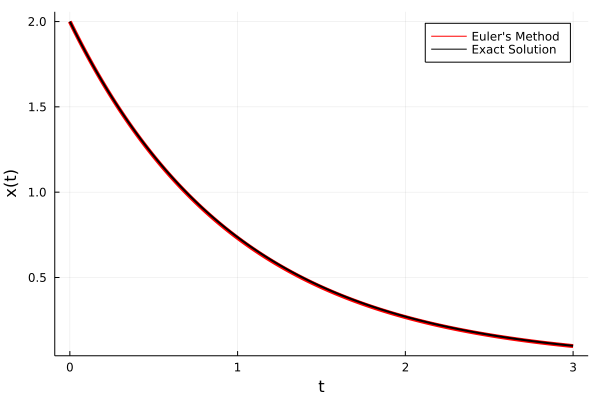
\includegraphics[width=0.6\columnwidth]{graphics/Chap09/FirstUseOfEulerMethod.png}
\end{center}

Wow! That's incredible, our computed Euler's numerical approximation to the ODE is indistinguishable from the true solution! Yeah, but we got lucky. For more complicated ODEs, you should really use better approximations than Euler's Method, but hey, this is ROB 101 and we just want to learn the basics. \\


In the above plot, we set $dt = 0.01$ seconds, or 10 ms. To see what we mean by getting lucky, let's increase the value of $dt$ by a factor of ten, namely, $dt = 0.1$ seconds. The resulting plot is still pretty satisfying, because we are still close to the true answer. The challenge is that in real engineering problems, we do not know the ``true answer'' and we're using numerical methods to  \textbf{``approximate it'' without having a closed-form answer against which to check how good of a job we are doing}. Here we still did OK. \\

\begin{lstlisting}[language=Julia,style=mystyle]
# first order linear differential equation
# dx/dt = - x
function SimpleOde(x)
    return - x
end

x0 = 2.0; t0 = 0.0; dt = 0.1; tf=3.0
N = 1 + floor(Int64,tf/dt) # want to return an integer
x = zeros(1,N); t = zeros(1,N)
x[1] = x0
t[1] = t0
for k = 1:(N-1)
    #xkp1 = xk + dt*f(xk)
    x[k+1] = x[k] + dt*SimpleOde(x[k])
    t[k+1] = t[k] + dt
end
y = x0*exp.(-t) # closed form solution

t=t';x=x';y=y' #for plotting 
p1 = plot(t,x, xlabel = "t", ylabel = "x(t)", lw=4, color = "red", labels = "Euler's Method" )
p1 = plot!(t, y, lw=2, color = "black", labels = "Exact Solution" )
png("UseOfEulerMethodLarge_dt")
display(p1)
\end{lstlisting}
\textbf{Output} 
\begin{center}
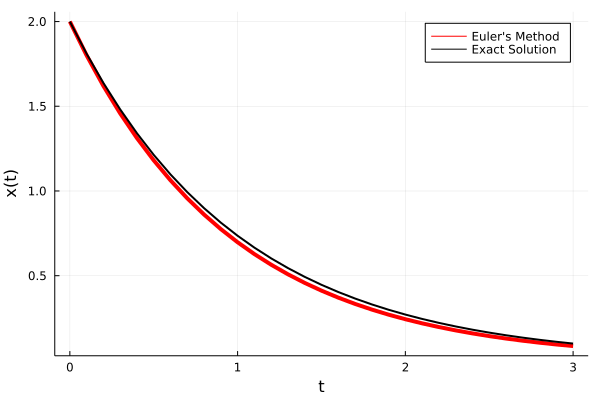
\includegraphics[width=0.6\columnwidth]{graphics/Chap09/UseOfEulerMethodLarge_dt.png}
\end{center}

The above shows that large values of $dt$ lead to errors even for simple ODEs. You might think that by taking $dt$ sufficiently small, you can always find a good approximation. That's not totally false, but (a) computing the solution will take a long time, and even more importantly, you can run into other ``numerical problems''. To learn more, you need to take the ODE course! \\

Next we compute a solution to a well-known linear oscillator,
\begin{equation}
\label{eq:LinearOscillator}
\begin{aligned}
  \dot{x}_1 &= x_2\\
  \dot{x}_2 & = -\pi^2 x_1,
\end{aligned}
\end{equation}
where Euler's method does a great job for several cycles, but then starts diverging from the true solution. We emphasize that more sophisticated numerical solution schemes for ODEs are well known and are routinely used in practice. Here, in ROB 101, we are just getting a taste for what is an ODE and how can one even conceive of computing solutions. \\

\begin{lstlisting}[language=Julia,style=mystyle]
# linear differential equation
# where x is a vector
#
# dx/dt = [x2; -pi^2 * x1]
function LessSimpleOde(x)
    return [x[2]; - pi^2*x[1]]
end

x0 = [0;pi]; t0 = 0.0; dt = 0.01; tf=10
dimX = length(x0)
N = 1 + floor(Int64,tf/dt) # want to return an integer
x = zeros(dimX,N); t = zeros(1,N)
x[:,1] = x0
t[1] = t0
for k = 1:(N-1)
    #xkp1 = xk + dt*f(xk)
    x[:,k+1] = x[:,k] + dt*LessSimpleOde(x[:,k])
    t[k+1] = t[k] + dt
end
y = [sin.(pi*t); pi*cos.(pi*t)] # closed form solution
#y = [cos.(pi*t);-pi*sin.(pi*t)] # closed form solution for x0=[1;0]

titre = "Red = numerical approx. and black = exact solution"
t=t';x=x'; y = y' # for plotting purposes

p1 = plot(t, x, xlabel = "t", ylabel = "x(t)", lw=4, color = "red", title = titre, legend = false)
p1 = plot!(t, y, lw=2, color = "black")

png("UseOfEulerMethodSinusoid")
display(p1)
\end{lstlisting}
\textbf{Output} 
\begin{center}
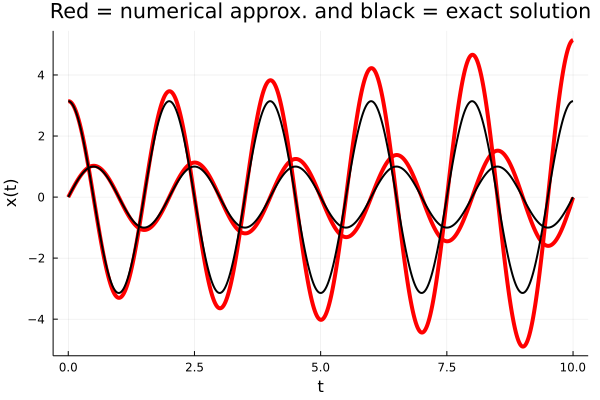
\includegraphics[width=0.6\columnwidth]{graphics/Chap09/UseOfEulerMethodSinusoid.png}
\end{center}
In the above solution, we took the initial condition as $t_0=0$ and
$$ x_0 = \begin{bmatrix} 0 \\ \pi \end{bmatrix}.
$$
For those who have taken Calc I, you can check that for this initial condition, 
\begin{align*}
    x(t) = \left[ \begin{array}{ll} x_1(t) \\ x_2(t) \end{array} \right]= \left[ \begin{array}{ll} \sin(\pi t) \\\pi \cos(\pi t) \end{array} \right]
\end{align*}
satisfies the initial condition $x(t_0)=x(0) = x_0 = \left[0~~~\pi\right]^\top$  and 
\begin{align*}
    \frac{d}{dt}x_1(t) & = \frac{d}{dt}\sin(\pi t)= \pi \cos(\pi t) = x_2(t)\\
     \frac{d}{dt}x_2(t) & = \frac{d}{dt}\pi \cos(\pi t)= -\pi^2 \sin(\pi t) = -\pi^2 x_1(t).
\end{align*}
This is what it means to be a solution to the ODE. Specifically, $x(t_0) = x_0$ and $\dot{x}(t) = f(x(t))$. If instead you take the initial condition as 
$$ x_0 = \begin{bmatrix} 1 \\ 0 \end{bmatrix},
$$
then $x_1(t) = \cos(\pi t)$ and $x_2(t) = -\pi \sin(\pi t)$
are the solution to the ODE. \\

Returning to the importance of numerical solutions of ODES, our point would be that no one knows a closed-form solution to the ODE $$ \dot{x}(t) = x_1(t) \cdot \cos(e^{x_1(t)}) - (x(t))^5, x(0)=-\sqrt{2},$$ and yet we can compute it numerically. \\


\begin{lstlisting}[language=Julia,style=mystyle]
# nonlinear differential equation
# 
#
# dx/dt = x * cos(exp(x)) - x^5
function NonlinearOde(x)
    return  x * cos(exp(x)) - x^5
end

x0 = -sqrt(2); t0 = 0.0; dt = 0.001; tf=2
N = 1 + floor(Int64,tf/dt) # want to return an integer
x = zeros(1,N); t = zeros(1,N)
x[1] = x0
t[1] = t0
for k = 1:(N-1)
    #xkp1 = xk + dt*f(xk)
    x[k+1] = x[k] + dt*NonlinearOde(x[k])
    t[k+1] = t[k] + dt
end

titre = "Red = numerical approx. and exact solut. unknown"
t=t'; x=x' # for plotting
p1 = plot(t, x, xlabel = "t", ylabel = "x(t)", lw=4, color = "red", title = titre, legend = false)
png("UseOfEulerMethodNonlinear")
display(p1)
\end{lstlisting}
\textbf{Output} 
\begin{center}
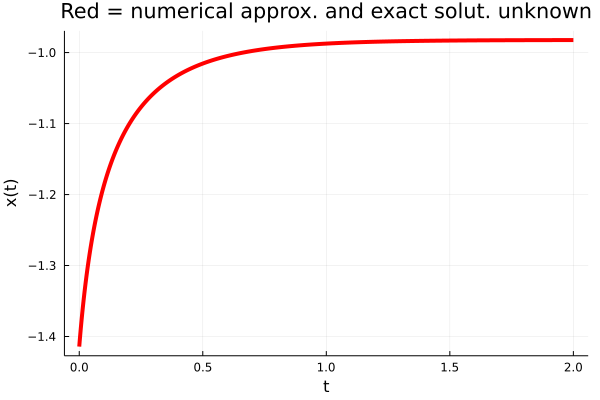
\includegraphics[width=0.6\columnwidth]{graphics/Chap09/UseOfEulerMethodNonlinear.png}
\end{center}

\section{Discrete-time Approximations of Continuous-time Linear ODEs with Control Variables}

A linear ODE with control variables is typically written as
\begin{equation}
\label{eq:LinearODE}
    \dot{x}(t) = A_c x(t) + B_c u(t),
\end{equation}
where $t\ge t_0$ represents time, $x(t) \in \real^n$ is the state vector, and $u(t) \in \real^m$ is a vector of control inputs, that is, the variables you can change by commanding motor torques, for example. From this information, you can deduce that $A_c$ is $n \times n$ and $B_c$ is $n \times m$. The initial value of the state is denoted $x_0 = x(t_0)$. We'll discuss how to make intelligent choices for the control signal in the next section.\\

To obtain a \textbf{discrete-time approximation} of the ODE \eqref{eq:LinearODE}, we use Euler's method and replace the time derivative with an approximation, 
\begin{equation}
\label{eq:LinearDT01}
    \frac{x(t + dt) - x(t)}{dt} = A_c x(t) + B_c u(t) \iff x(t+dt) = x(t) + dt \cdot(A_cx(t) + B_c u(t)).
\end{equation}
If for $k= 0, 1, 2, ...$ we define $t_k := t_0 + k dt$, $x_k := x(kt)$, $u_k := u(kt)$, we obtain
\begin{equation}
\label{eq:LinearDT02}
\begin{aligned}
   x_{k+1} &= x_k + dt\cdot A_c x_k + dt\cdot B_c u_k \\
   x_{k+1} &= \underbrace{(I + dt \cdot A_c)}_{A} x_k + \underbrace{dt\cdot B_c}_{B} u_k \\
    x_{k+1} & = A x_k + B u_k,
\end{aligned}
\end{equation}
where, $A:= I + dt \cdot A_c$ and $B := dt\cdot B_c$ are $n\times n$ and $n \times m$, respectively.\\

 \begin{figure}[hbt!]%
	\centering
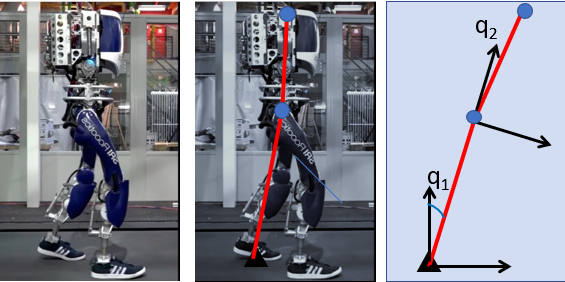
\includegraphics[width=0.75\columnwidth]{graphics/Chap09/Robot2PendulaVer02.png}
    \caption[]{Left is the bipedal robot, Durus, from Prof. Ames' group at Caltech. Center is a crude pendulum approximation of the robot. Right is a double inverted pendulum that we will balance in this lab! We assume the bottom link is actuated via a motor, while the middle link is a frictionless revolute joint. All angles are positive when measured clockwise from the vertical axis. A linear approximation of the double inverted pendulum's ODE model is given in \eqref{eq:LinearizedDoubleInvertedPendulum}.}
    \label{fig:FromRobots2Pendula}
\end{figure} 

\begin{tcolorbox}[title=\textbf{Euler's Method takes us from a Linear ODE to Iterating Linear Equations}]

A typical linear ODE looks like this.
 $$\dot{x}(t) = A_c x(t) + B_c u(t).$$
 With Euler's Method, we quickly approximate $\dot{x}(t)$ via
 $$  \frac{x(t + dt) - x(t)}{dt} = A_c x(t) + B_c u(t).$$
When for $k= 0, 1, 2, ...$ we define $t_k := t_0 + k dt$, $x_k := x(kt)$, $u_k := u(kt)$, we obtain 
$$  x_{k+1}  = A x_k + B u_k,$$
where $A:= I + dt \cdot A_c$ and $B:= dt \cdot B_c$, 
which we can solve with a \texttt{for\,loop}.
\end{tcolorbox}

\textbf{Why is Euler's method important?} A scary ODE now looks like one of our iterative algorithms, say the Bisection Method, Newton's Algorithm, or Gradient Descent. Once we convert the ODE \eqref{eq:LinearODE} into a discrete-time model \eqref{eq:LinearDT02}, we can compute solutions just by iterating with a \texttt{for\,loop}, which is quite remarkable. We'll illustrate this on a \textbf{double inverted pendulum} that approximates a legged robot; see Fig.~\ref{fig:FromRobots2Pendula}. Here is a linear ODE model that is valid for small deviations of the angles from zero, where $x_1 = q_1$ and $x_2 = q_2$ are the two angles of the pendula in radians and  $x_3 = \dot{q}_1$ and $x_4 = \dot{q}_2$ are the angular rates in radians per second. 
\begin{equation}
\label{eq:LinearizedDoubleInvertedPendulum}
 \underbrace{ \left[
\begin{array}{r}
\dot{x}_1(t) \\
\dot{x}_2(t) \\
\dot{x}_3(t) \\
\dot{x}_4(t) \\
\end{array}
\right]}_{\dot{x}(t)} = \underbrace{\left[
\begin{array}{rrrr}
0.0000 & 0.0000 & 1.0000 & 0.0000 \\
0.0000 & 0.0000 & 0.0000 & 1.0000 \\
39.2400 & -31.3920 & 0.0000 & 0.0000 \\
-78.4800 & 133.4160 & 0.0000 & 0.0000 \\
\end{array}
\right]}_{A_c} \underbrace{\left[
\begin{array}{r}
x_1(t) \\
x_2(t) \\
x_3(t) \\
x_4(t) \\
\end{array}
\right]}_{x(t)} + \underbrace{\left[
\begin{array}{r}
0.0000 \\
0.0000 \\
3.2000 \\
-9.6000 \\
\end{array}
\right]}_{B_c} u(t).
\end{equation}

If we take $dt = 0.1$, then the associated discrete-time model becomes 
 \begin{equation}
\label{eq:DTLinearizedDoubleInvertedPendulum}
 \underbrace{ \left[
\begin{array}{r}
x_{1,k+1} \\
x_{2,k+1}  \\
x_{3,k+1}  \\
x_{4,k+1}  \\
\end{array}
\right]}_{x_{k+1}} = \underbrace{\left[
\begin{array}{rrrr}
1.0000 & 0.0000 & 0.1000 & 0.0000 \\
0.0000 & 1.0000 & 0.0000 & 0.1000 \\
3.9240 & -3.1392 & 1.0000 & 0.0000 \\
-7.8480 & 13.3416 & 0.0000 & 1.0000 \\
\end{array}
\right]}_{A} \underbrace{\left[
\begin{array}{r}
x_{1,k} \\
x_{2,k}  \\
x_{3,k}  \\
x_{4,k}  \\
\end{array}
\right]}_{x_k} + \underbrace{\left[
\begin{array}{r}
0.0000 \\
0.0000 \\
0.3200 \\
-0.9600 \\
\end{array}
\right]}_{B} u_k.
\end{equation}

\begin{lstlisting}[language=Julia,style=mystyle]
using LinearAlgebra
# Linear Double Inverted Pendulum Model 
F=dyn_mod_2LinkPendulum([0;0],[0;0])
A11=zeros(2,2);   A22=zeros(2,2)
A12=zeros(2,2)+I; A21=-inv(F.D)*F.JacG
#
# Continuous-time terms in the ODE model
Ac = [A11 A12;A21 A22]
Bc = [zeros(2,1);inv(F.D)*F.B]

# Discrete time model
dt = 0.1
A = I + dt*Ac
B = dt*Bc;
\end{lstlisting}

We now compute the evolution of the double inverted pendulum when the initial condition does not correspond to the upright equilibrium position and the motor torque is identically zero. \\

\begin{lstlisting}[language=Julia,style=mystyle]
# Run me, don't change me
x0=[pi/16; -pi/16; 0; 0]
t0 = 0.0; tf=1
N = 1 + floor(Int64,tf/dt) # want to return an integer
x = zeros(length(x0),N); t = zeros(1,N)
x[:,1] = x0
t[1] = t0
for k = 1:(N-1)
    #xkp1 = xk + dt*f(xk)
    x[:,k+1] = A*x[:,k]
    t[k+1] = t[k] + dt
end
\end{lstlisting}
\textbf{Output} 
\begin{figure}[htb!]%
\centering
\subfloat[]{%
     
	\centering
		\setlength{\fboxsep}{0pt}%
\setlength{\fboxrule}{3pt}%
	\fbox{
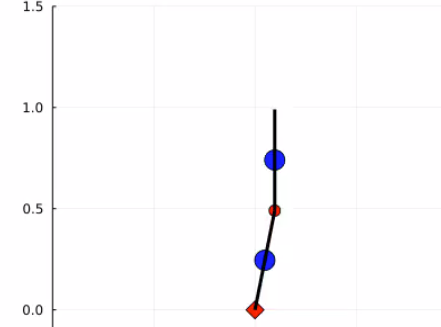
\includegraphics[width=0.43\columnwidth]{graphics/Chap09/OLpendulumteq0pt0.png}}%
}
\hspace{20pt }%
\subfloat[]{%
    \label{fig:LiDARmap}%
	\centering
	\setlength{\fboxsep}{0pt}%
\setlength{\fboxrule}{3pt}%
\fbox{
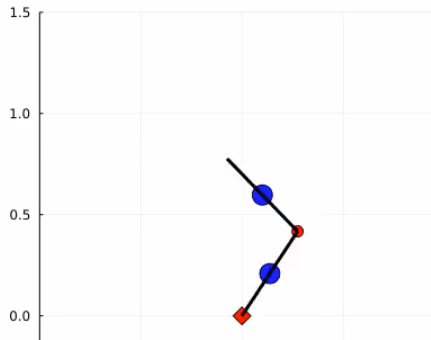
\includegraphics[width=0.405\columnwidth]{graphics/Chap09/OLpendulumteq0pt1.png}}%
}
\hspace{20pt }%
\subfloat[]{%
     
	\centering
		\setlength{\fboxsep}{0pt}%
\setlength{\fboxrule}{3pt}%
	\fbox{
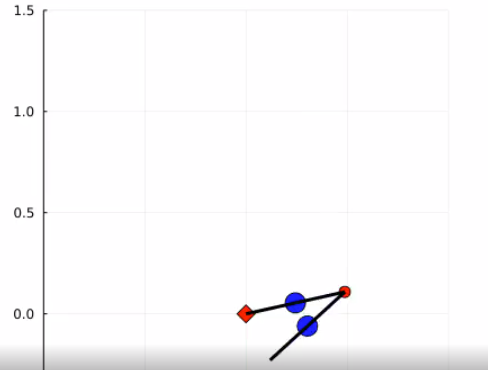
\includegraphics[width=0.435\columnwidth]{graphics/Chap09/OLpendulumteq0pt2.png}}%
}
\hspace{20pt }%
\subfloat[]{%
     
	\centering
		\setlength{\fboxsep}{0pt}%
\setlength{\fboxrule}{3pt}%
	\fbox{
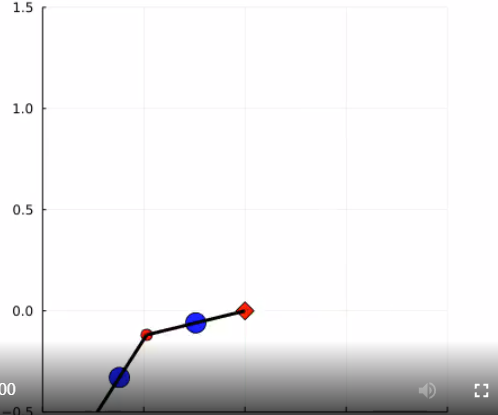
\includegraphics[width=0.4\columnwidth]{graphics/Chap09/OLpendulumteq0pt3.png}}%
}

\caption[]{Evolution of the double inverted pendulum when $u_k \equiv 0.0$. The images are the pendulum's configurations at $t_0=0.0$, $t_1=0.1$, $t_2=0.2$ and $t_3=0.3$ seconds. Without the proper inputs, the pendulum falls over. Are we surprised?}
    \label{fig:SnapShotFallingPendulum}
\end{figure}

Just for fun, we give the nonlinear model of the double inverted pendulum. Your author generated it using Lagrangian mechanics, a technique that is taught in advanced Physics courses or advanced ME courses on dynamics. 

\begin{lstlisting}[language=Julia,style=mystyle]
function   dyn_mod_2LinkPendulum(q,dq)
#DYN_MOD_2LINKPENDULUM
#20-Jun-2022 12:32:57
#
# Author: Grizzle
#
#
# Model NOTATION: Spong and Vidyasagar, page 142, Eq. (6.3.12)
#                 D(q)*ddq + C(q,dq)*dq + G(q) = B*tau 
#
#
g,L1,L2,m1,m2=modelParameters();
#
#
#
#
q1=q[1];q2=q[2];
dq1=dq[1];dq2=dq[2];
#
#
#
#
D=zeros(2,2);
D[1,1]=(m2*(8*L1^2 + 2*L2^2 + 8*L1*L2*cos(q2)))/8 + (L1^2*m1)/4;
D[1,2]=(L2*m2*(L2 + 2*L1*cos(q2)))/4;
D[2,1]=(L2*m2*(L2 + 2*L1*cos(q2)))/4;
D[2,2]=(L2^2*m2)/4;
#
#
#
#
C=zeros(2,2);
C[1,1]=-(L1*L2*dq2*m2*sin(q2))/2;
C[1,2]=-(L1*L2*m2*sin(q2)*(dq1 + dq2))/2;
C[2,1]=(L1*L2*dq1*m2*sin(q2))/2;
#
#
#
#
G=zeros(2,1);
G[1]=- g*m2*((L2*sin(q1 + q2))/2 + L1*sin(q1)) - (L1*g*m1*sin(q1))/2;
G[2]=-(L2*g*m2*sin(q1 + q2))/2;
#
#
#
#
B=zeros(2,1);
B[1,1]=1;
#
#
JacG=zeros(2,2);
JacG[1,1]=- g*m2*((L2*cos(q1 + q2))/2 + L1*cos(q1)) - (L1*g*m1*cos(q1))/2;
JacG[1,2]=-(L2*g*m2*cos(q1 + q2))/2;
JacG[2,1]=-(L2*g*m2*cos(q1 + q2))/2;
JacG[2,2]=-(L2*g*m2*cos(q1 + q2))/2;
#
#
return (D=D,C=C,G=G,B=B,JacG=JacG)
end
\end{lstlisting}

\section{Predicting the State Vector at Future Instants of Time}

Now that we have a means to compute the state at the next time instance based on the current state and current input, we can also iterate forward and \textbf{predict the state at some future time}, say $N$ steps ahead, as a function of a hypothesized input sequence, $\{u_0, u_1, \ldots, u_{N-1} \}$, as follows
\begin{align}
    x_0 &= \text{ given} \nonumber\\
    x_1 &= A x_0 + B u_0 \nonumber\\
    x_2 &= A x_1 + B u_1 = A(A x_0 + B u_0 ) + B u_1 = A^2 x_0 + A B u_0 + B u_1 \nonumber\\
    x_3 &= A x_2 + B u_2 = A(A^2 x_0 + A B u_0 + B u_1) + B u_2 = A^3 x_0 + A^2 B u_0 + A B u_1 + B u_2 \nonumber\\
    &\vdots \nonumber\\
    x_N &= A^N x_0 + A^{N-1} B u_0 + A^{N-2} B u_1 + \cdots + A B u_{N-2} + B u_{N-1} \label{eq:stateTransition_derive_init}
\end{align}

\textbf{We now focus on that last line of \eqref{eq:stateTransition_derive_init}. We will see that it is a gold mine.} We note that
\begin{align}
       x_N &=  A^N x_0 + A^{N-1} \cdot B u_0 + A^{N-2} \cdot B u_1 + \cdots + A \cdot B u_{N-2} + B u_{N-1}\\
       x_N&=  \underbrace{A^N}_{S}x_0+ \underbrace{\left[\begin{array}{ccccc} A^{N-1} \cdot B  & A^{N-2} \cdot B & \cdots & A\cdot B & B \end{array} \right]}_{M} \cdot  \underbrace{\left[\begin{array}{c} u_0 \\ u_1 \\  \vdots \\ u_{N-2} \\ u_{N-1} \end{array} \right]}_{u_{\rm seq}},
       \label{eq:stateTransition_derive}
\end{align}
where for compactness of notation, we define
\begin{align}
\label{eq:CompactFormula01}
S&:= A^N \\
\label{eq:CompactFormula02}
M &:=\left[\begin{array}{ccccc} A^{N-1} \cdot B  & A^{N-2} \cdot B & \cdots & A\cdot B & B \end{array} \right], \text{~~and~~}  \\
\label{eq:CompactFormula3}
u_{\rm seq}&:=\left[\begin{array}{l} u_0 \\ u_1 \\  ~~\vdots \\ u_{N-2} \\ u_{N-1}, \end{array} \right].
\end{align}
\textbf{This leads to our most important equations so far:}
\begin{equation}
    \label{eq:GoldMine}
\boxed{\begin{aligned}
   x_N &= S x_0 + M u_{\rm seq} \\
   & \Updownarrow \\
    x_N - S x_0 &= M u_{\rm seq}  \\
      & \Updownarrow \\
    M u_{\rm seq} &= (x_N - S x_0).
\end{aligned}}
\end{equation}
\textbf{If the rows of $M$ are linearly independent}, then we can solve for a vector $u_{\rm seq}$ of minimum norm that satisfies \eqref{eq:GoldMine} using our knowledge of underdetermined linear equations. We illustrate this on our discrete-time model of the double inverted pendulum in \eqref{eq:DTLinearizedDoubleInvertedPendulum}.




% \begin{lstlisting}[language=Julia,style=mystyle]

% \end{lstlisting}
% \textbf{Output} 
% \begin{verbatim}

% \end{verbatim}




% \begin{lstlisting}[language=Julia,style=mystyle]

% \end{lstlisting}
% \textbf{Output} 
% \begin{verbatim}

% \end{verbatim}

\begin{lstlisting}[language=Julia,style=mystyle]
N=8
x0=[pi/16; -pi/16; 0; 0]
t0=0

# Predict ahead
S=A^N
M=B
for k = 1:N-1
    M=[A*M B]
end

xGoal = [0.;0.;0.;0.]
# Solve for input such that x[N]=xGoal using least squares
if true
    # Cheating method to solve least squares..we use the inverse function :( oh no....
    useq = (M') * inv(M*(M')) * (xGoal-S*x0)
else # better way to do it
    useq = minNormUnderdetermined(M,xGoal-S*x0)
end
# Verify we have a good solution
@show xGoal
@show xFinal=S*x0+M*useq
#
# Now, solve for x[k], 0 <= k <= N
x = zeros(length(x0),N+1); t = zeros(1,N+1)
x[:,1]=x0
for k = 1:N
    x[:,k+1] = A*x[:,k] + B*useq[k]
    t[k+1] = t[k] + dt
end
@show x[:,end]
animateInvPendulum(x)
\end{lstlisting}
\textbf{Output} 
\begin{verbatim}
xGoal = [0.0, 0.0, 0.0, 0.0]
xFinal = S * x0 + M * useq = 
[6.481984013362307e-5, -0.00020456325910345186, 0.0014950509685149882, -0.004721057710412424]
x[:, end] = [6.481984022717204e-5, -0.00020456325908854315, 0.0014950509688680391,
-0.004721057705593168]
\end{verbatim}


\textbf{Snapshots of the pendulum's evolution are given in Fig.~\ref{fig:SnapShotBalancingPendulum}}.

\vspace*{.6cm}

\textbf{Remark:} The least squares solution to underdetermined equations is studied in Chapter 9 of our textbook. The key results are as follows: Consider an underdetermined system of linear equations $M u_{\rm seq}=x_{\rm Goal}-S x_k$. If the rows of $M$ are linearly independent (equivalently, the columns of $M^\top$ are linearly independent), then 
\begin{equation}
\label{eq:MinNormUnderDetermined}
    u_{\rm seq}^\ast = \argmin_{M u_{\rm seq}=(x_{\rm Goal}-S x_k)} ||u_{\rm seq}||^2  \iff u_{\rm seq}^\ast= M^\top \alpha~~\text{and}~~M\cdot M^\top \alpha = \left(x_{\rm Goal}-S x_k\right).
\end{equation}
We do the QR Factorization of $M^\top$ instead of $M$ itself, so that
$$ M^\top = Q \cdot R.$$
Then, 
\begin{equation}
\label{eq:MinNormUnderDeterminedQR}
    u_{\rm seq}^\ast = \argmin_{M u_{\rm seq}=(x_{\rm Goal}-S x_kb)} ||u_{\rm seq}||^2  \iff u_{\rm seq}^\ast = Q \beta~~\text{and}~~R^\top \beta = \left(x_{\rm Goal}-S x_k \right).
\end{equation}
We note that $R^\top$ is lower triangular, and thus $R^\top \beta = \left(x_{\rm Goal}-S x_k \right)$ can be solved via forward substitution. See Chapter 9 for more details. 
\newpage

\begin{figure}[htb!]%
\centering
\subfloat[]{%
     
	\centering
		\setlength{\fboxsep}{0pt}%
\setlength{\fboxrule}{3pt}%
	\fbox{
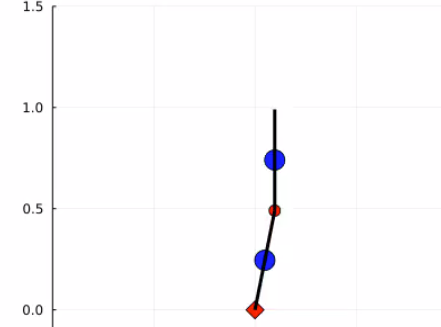
\includegraphics[height=0.250\columnwidth]{graphics/Chap09/OLpendulumteq0pt0.png}}%
}
\hspace{20pt }%
\subfloat[]{%
    \label{fig:LiDARmap}%
	\centering
	\setlength{\fboxsep}{0pt}%
\setlength{\fboxrule}{3pt}%
\fbox{
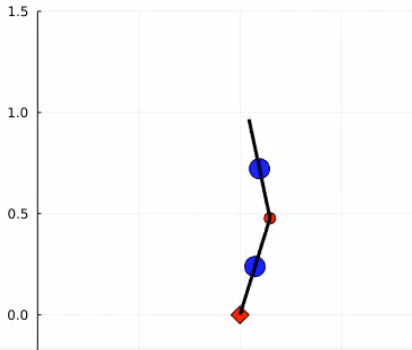
\includegraphics[height=0.250\columnwidth]{graphics/Chap09/CLpendulumteq0pt1.png}}%
}
\hspace{20pt }%
\subfloat[]{%
     
	\centering
		\setlength{\fboxsep}{0pt}%
\setlength{\fboxrule}{3pt}%
	\fbox{
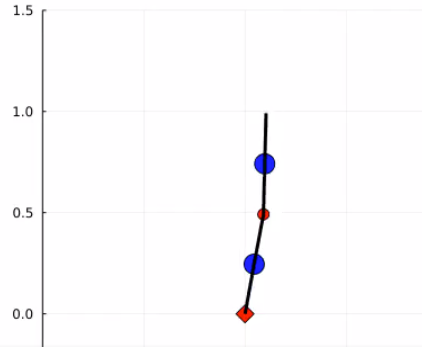
\includegraphics[height=0.250\columnwidth]{graphics/Chap09/CLpendulumteq0pt2.png}}%
}
\hspace{20pt }%
\subfloat[]{%
     
	\centering
		\setlength{\fboxsep}{0pt}%
\setlength{\fboxrule}{3pt}%
	\fbox{
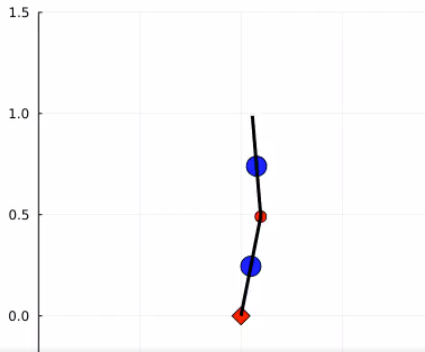
\includegraphics[height=0.250\columnwidth]{graphics/Chap09/CLpendulumteq0pt3.png}}%
}

\subfloat[]{%
     
	\centering
		\setlength{\fboxsep}{0pt}%
\setlength{\fboxrule}{3pt}%
	\fbox{
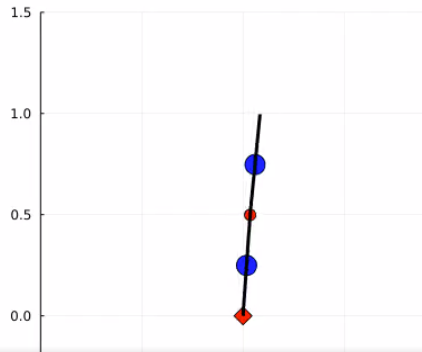
\includegraphics[height=0.250\columnwidth]{graphics/Chap09/CLpendulumteq0pt4.png}}%
}
\hspace{20pt }%
\subfloat[]{%
    \label{fig:LiDARmap}%
	\centering
	\setlength{\fboxsep}{0pt}%
\setlength{\fboxrule}{3pt}%
\fbox{
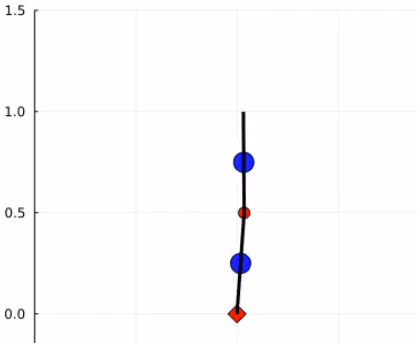
\includegraphics[height=0.250\columnwidth]{graphics/Chap09/CLpendulumteq0pt5.png}}%
}
\hspace{50pt}%
\subfloat[]{%
     
	\centering
		\setlength{\fboxsep}{0pt}%
\setlength{\fboxrule}{3pt}%
	\fbox{
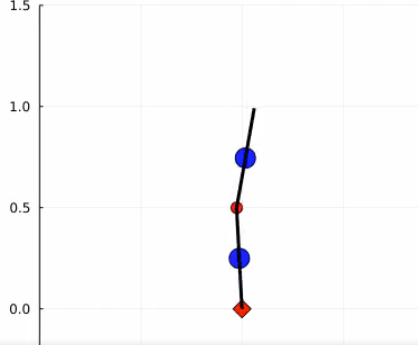
\includegraphics[height=0.250\columnwidth]{graphics/Chap09/CLpendulumteq0pt6.png}}%
}
\hspace{20pt }%
\subfloat[]{%
     
	\centering
		\setlength{\fboxsep}{0pt}%
\setlength{\fboxrule}{3pt}%
	\fbox{
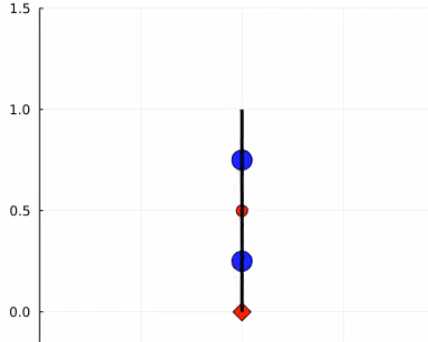
\includegraphics[height=0.250\columnwidth]{graphics/Chap09/CLpendulumteq0pt7.png}}%
}

\caption[]{Evolution of the double inverted pendulum when the sequence $u_0, \ldots, u_7$ is chosen to drive the pendulum to the upright position. The images are the pendula's configurations at $t_0=0.0$, $t_1=0.1$, $t_2=0.2$, ..., $t_7=0.7$ seconds. With the proper inputs, the pendulum balances nicely. Are we happy?}
    \label{fig:SnapShotBalancingPendulum}
\end{figure}

\begin{lstlisting}[language=Julia,style=mystyle]
# The QR pipeline for minimum norm solution of Ax=b when
# the ROWS of A are linearly independent 
# (yes, the columns of A' are linearly independent)

function forwardsub(L, b)    
    (nr,nc) = size(L)
    x = Vector{Float64}(undef,nc)
    if minimum(abs.(diag(L))) < 1e-8
        println("L is close to singular. I will not solve this problem")
        return x
    else    
        x[1] = b[1] / L[1,1]
        for i = 2:nc
            x[i]=( b[i] - L[i,1:i-1]' * x[1:i-1] ) ./ L[i,i]
        end
        return x  
    end
end

# Call me with A = M and b = (xGoal - Sxk)
function minNormUnderdetermined(A,b)
    # Solves for minimum norm x in Ax = b 
    # using the QR factorization and forward substitution. Returns xStar.
    # xStar = arg min x' x
    #  subject to  Ax = b
    F = qr(A')
    Q = Matrix(F.Q)
    R = Matrix(F.R)
    beta = forwardsub(R', b) 
    xStar = Q*beta
    return xStar
end
\end{lstlisting}
\textbf{Output} 
\begin{verbatim}
minNormUnderdetermined (generic function with 1 method)
\end{verbatim}

\section{(Optional Read:) For What Values of $N$ are the Rows of $M$ Linearly Independent? }

We write a simple script to check for the rows of $M:=[A^{N-1}\cdot B~~ \cdots ~~A\cdot B~~~B]$ to be linearly independent.\\

\begin{lstlisting}[language=Julia,style=mystyle]
for N = 1:10
    M=B
    for k = 1:N-1
        M=[A*M B]
    end
    detMMtrans = det(M*M')
    rankM = rank(M,rtol=1e-6)
    println("For N = $N, det(M*M') = $detMMtrans,   rank(M) = $rankM")   
end
\end{lstlisting}
\textbf{Output} 
\begin{verbatim}
For N = 1, det(M*M') = 0.0,   rank(M) = 1
For N = 2, det(M*M') = -5.816113682013453e-32,   rank(M) = 2
For N = 3, det(M*M') = -2.294447422015386e-17,   rank(M) = 3
For N = 4, det(M*M') = 0.001629280421367469,   rank(M) = 4
For N = 5, det(M*M') = 0.13025026505817638,   rank(M) = 4
For N = 6, det(M*M') = 9.088750148559221,   rank(M) = 4
For N = 7, det(M*M') = 431.06039658516085,   rank(M) = 4
For N = 8, det(M*M') = 19417.82334475286,   rank(M) = 4
For N = 9, det(M*M') = 772663.0420936232,   rank(M) = 3
For N = 10, det(M*M') = 3.0107394769364707e7,   rank(M) = 3
\end{verbatim}

The ``theoretically correct'' result is that for all $N\ge 1$, $\rank(M) = \min\{N,4\}$. As we see, the ``numerical rank'' of $M$ ``deteriorates'' for $N > 8$. Hence, our value of $N=8$ used for Fig.~\ref{fig:SnapShotBalancingPendulum} now makes more sense.

\section{Feedback Control of Discrete-time Linear Models via Least Squares for Underdetermined Systems of Equations}

In this section, we get very close to real Robotics. 

\subsection{Getting the Pendulum Upright is not Enough} 

To get started, we need to observe that the final value of the state $x$ in Fig.~\ref{fig:SnapShotBalancingPendulum} is nearly zero, but is not exactly equal to zero,
$$ x_{\rm final} \approx [6.48e\text{-}5, -0.0002, 0.001495,-0.0047]. $$
Since the pendulum is not exactly at the equilibrium, it will fall once we are no longer providing inputs that strive to keep it upright, as the next code block verifies. If we continue computing $x(kdt)$ for $ 8 < k \le 16$ with $u_k=0$, we end up with $x(16dt)\approx  [0.94, -2.97, 21.72, -68.59] $. Oopps! The pendulum falls. \\

Even if we had achieved $x_{\rm final} \equiv [0.0, 0.0, 0.0, 0.0],$ and thus the pendula are in prefect equilibrium, would that be enough? What would happen if a slight gust of air passed over the device? Or a slight vibration of the platform on which the device is setting caused it to wiggle just a tiny bit? Or what if the parameters in the model that were used for computing $u_{\rm seq}$ were just a bit different than the real device? In all of these cases, the pendula would fall. 

\vspace*{.2cm}


\begin{lstlisting}[language=Julia,style=mystyle]
# Here we simulate for longer than we control
N=8 # Planning horizon
x0=[pi/16; -pi/16; 0; 0]
t0=0
Nsim = 16  # Simulation duration
# Predict ahead
S=A^N
M=B
for k = 1:N-1
    M=[A*M B]
end

xGoal = [0.;0.;0.;0.]
# Solve for input such that x[N]=xGoal using least squares
if true
    # Cheating method to solve least squares..we use the inverse function :( oh no....
    useq = (M') * inv(M*(M')) * (xGoal-S*x0)
else # better way to do it
    useq = minNormUnderdetermined(M,xGoal-S*x0)
end
# Verify we have a good solution
@show xGoal
@show xFinal=S*x0+M*useq
#
# Now, solve for x[k], 0 <= k <= N
x = zeros(length(x0),Nsim+1); t = zeros(1,Nsim+1)
x[:,1]=x0

for k = 1:Nsim
    if k > N
        x[:,k+1] = A*x[:,k]  # uk = 0
    else
        x[:,k+1] = A*x[:,k] + B*useq[k]
    end
    t[k+1] = t[k] + dt
end
@show x[:,end]
animateInvPendulum(x)
\end{lstlisting}
\textbf{Output} 
\begin{verbatim}
xGoal = [0.0, 0.0, 0.0, 0.0]
xFinal = S * x0 + M * useq = 
[6.481984013362307e-5, -0.00020456325910345186, 0.0014950509685149882,
-0.004721057710412424]
[N Nsim] = [8 16]
x[:, end] = [0.93888952433862, -2.965304039678654, 21.715899365969108, -68.5855850968567]
\end{verbatim}

\vspace*{.2cm}

\subsection{Keeping the Pendulum Upright is Our Goal}

Let's summarize what we  have learned so far:
\begin{itemize}
    \item If we choose a fixed number of time steps, $N_{\rm horiz}$, large enough so that the rows of $M$ are linearly independent, we know theoretically how to compute a sequence of control values 
    $$u_{\rm seq} = u_0, u_1, \ldots, u_{N_{\rm horiz -1}} $$
    that drives the pendulum from an initial condition $x_0$ to a goal state that we are choosing as the upright equilibrium for the double inverted pendulum.
    \item In our numerical simulations, even for the linear model, our calculations have a small amount of numerical error so that $u_{\rm seq}$ does not drive the double inverted pendulum to the exact equilibrium. We get close, but if we continue the computation of the solution of the double inverted pendulum with zero as the control input, it tips over and falls. The same thing would happen on a real robot, by the way, so our issue is not limited to numerical simulations.
    \item We chose $N_{\rm horiz}=8$. One possibility is to make it bigger, say 16, or 20, or why not 100? Well, no matter how big we make it, the pendulum will fall over when our control sequence ends.  
    \item Also, our control sequence is computed on the basis of our linear model, which we are assuming to be correct. If the pendula were perturbed by a person, or by wind, or by friction in the joints, then our predicted behavior from the model would be incorrect. You can check that these scenarios once again lead to the pendula falling. 
    \item If you are thinking that well, we could measure $x_{N_{\rm horiz}}$, compute a new control sequence $u_{\rm seq}$, apply it for the next $N_{\rm horiz}$ time steps, and repeat this process, then you have just invented what is called \textbf{Model Predictive Control or MPC for short}!
\end{itemize}

\begin{tcolorbox}[title=\textbf{\large From $x_k$ to $x_{k+N}$ as a function of the control sequence.}]

What happens if you know the state at time $k$ and want to predict its value at some future time $k+N$? It works like this
\begin{equation}
x_{k+N} = S x_k + M u_{\rm seq}, 
    \label{eq:GoldMine2}
\end{equation}
where this time, 
$$u_{\rm seq}:=\left[\begin{array}{l} u_k \\ u_{k+1} \\~~  \vdots \\ u_{k+N-2} \\ u_{k+N-1} \end{array} \right], $$
while $S$ and $M$ are still given by \eqref{eq:CompactFormula01} and \eqref{eq:CompactFormula02}.
\textbf{In other words, the formula does not change.} 
\end{tcolorbox}

\vspace*{.2cm}

\textbf{The fix for the falling pendulum is to compute new controls that drive the pendulum to its goal state, the upright equilibrium.} In the modern version of Model Predictive Control, aka MPC, we do not wait the full $N_{\rm horiz}$ time steps before computing a new control sequence, $u_{\rm seq}$. Instead, \textbf{at each instant of time $k dt$}, we measure the current state $x_k$ of the double pendulum, compute a new sequence of control commands, $u_{\rm seq} = [u_k, u_{k+1}, \ldots, u_{k+N_{\rm horiz}-1}]$, for the given horizon length, $N_{\rm horiz}$, that steers the double inverted pendulum to its equilibrium, \textbf{apply the first value in the sequence which gets us to time step $(k+1)dt$}, and repeat the process all over again (means, put this process in a \texttt{for\,loop}). 

\vspace*{.2cm}

\begin{tcolorbox}[sharp corners, colback=green!30, colframe=green!80!blue, title=\textbf{MPC: Closed-loop Control via Least-squares Optimization }]
Model Predictive Control works as follows. 
\begin{enumerate}
 \renewcommand{\labelenumi}{(\alph{enumi})}
\setlength{\itemsep}{.1cm}   
\item Set a goal, $x_{\rm Goal}$.
\item Set a (relatively short-term) planning horizon for control, consisting of $N_{\rm horiz}$ time steps;
\item \textbf{ \large FOR $k=0:N_{ \text{ as long as you want to balance the pendula} }$ }
\begin{itemize}
\setlength{\itemsep}{.1cm}
\item measure the system's current state, $x_k$;
\item using \eqref{eq:MinNormUnderDeterminedQR}, solve $$u_{\rm seq}^\ast:= \argmin_{M u_{\rm seq} =\left(x_{\rm Goal} - S x_k\right)} ||u_{\rm seq}||^2,$$ where $S$ and $M$ are given in \eqref{eq:CompactFormula01} and \eqref{eq:CompactFormula02} with $N=N_{\rm horiz}$;  
\item define $u_k:= u_{\rm seq}[1]$ and apply it to the actuators of your system (that is, the motor driving the base of the double inverted pendulum).
\item Either let physics do its thing and compute $x_{k+1}$ for you, or, in the case of a computer simulation, apply the control $u_k$ to your mathematical model to compute $x_{k+1} = A x_k + Bu_k$, and then wash, rinse, and repeat.
\end{itemize}
\textbf{\large END}
\end{enumerate}
\end{tcolorbox}

\subsection{Relevant Code for MPC}
 
Here we give code that supports MPC control. 

\vspace*{.2cm}


\begin{lstlisting}[language=Julia,style=mystyle]
function myMPC(A,B,xk,nControlHoriz,xGoal)
    # xk is the current position and velocity of the pendulum links
    # k is the time index. Hence, tk = k dt
    (nr,nc) = size(A)
    nControlHoriz=max(nControlHoriz,nr)  # Cannot be smaller than nr
    S=A^nControlHoriz
    M=Array{Float64,2}(undef,nr,0)
    for i=1:nControlHoriz
        M=[A*M B]
    end
    C=zeros(nr,nr)+I
    uControl=minNormUnderdetermined(C*M,C*(xGoal-S*xk))
    uk=uControl[1]
    return uk
end
\end{lstlisting}
\textbf{Output} 
\begin{verbatim}
myMPC (generic function with 1 method)
\end{verbatim}

The next code block simulates the linear system $x_{k+1} = A x_k + B u_k$ under MPC control.\\

\begin{lstlisting}[language=Julia,style=mystyle]
function LinSimMPC(A,B,x0,nControlHoriz,Nsim,xGoal)
    (rA,cA) = size(A)
    N=1+Nsim # because x0 is included
    xTraj = Array{Float64,2}(undef,rA,0)
    uTraj = Array{Float64,2}(undef,1,0)
    xTraj=[xTraj x0]
    for k = 1:N
        xk=xTraj[:,k]
        uk=myMPC(A,B,xk,nControlHoriz,xGoal)
        uTraj=[uTraj uk]
        xkp1 = A*xk+B*uk
        xTraj = [xTraj xkp1]          
    end
    return (xTraj=xTraj, uTraj=uTraj)
end
\end{lstlisting}
\textbf{Output} 
\begin{verbatim}
LinSimMPC (generic function with 1 method)
\end{verbatim}

The next code block simulates a nonlinear system $x_{k+1} = x_k + dt f(x_k, u_k)$ under MPC control.\\

\begin{lstlisting}[language=Julia,style=mystyle]
# 2 link inverted pendulum
function f(x1,x2,u=[0.0])
    F=dyn_mod_2LinkPendulum(x1,x2)
    Kfric=0*diagm([.1;.1])
    # Use the backslash command to solve for x2 dot
    dx2=F.D\(-F.C*x2-F.G-Kfric*x2+F.B*u)
    return dx2
end

# Apply our linear MPC solution to the real nonlinear model

function NonLinSimMPC(f,dt,A,B,x0,nControlHoriz,Nsim,xGoal)
    rA = length(x0)
    N=1+Nsim # because x0 is included
    xTraj = Array{Float64,2}(undef,rA,0)
    uTraj = Array{Float64,2}(undef,1,0)
    xTraj=[xTraj x0]
    for k = 1:N
        xk=xTraj[:,k]
        uk=myMPC(A,B,xk,nControlHoriz,xGoal)
        uTraj=[uTraj uk]
        dx2 = f(xk[1:2],xk[3:4],uk)
        xkp1 = xk + dt*[xk[3:4];dx2]
        xTraj = [xTraj xkp1]          
    end
    return (xTraj=xTraj, uTraj=uTraj)
end
\end{lstlisting}
\textbf{Output} 
\begin{verbatim}
NonLinSimMPC (generic function with 1 method)
\end{verbatim}

\subsection{Balancing the Double Inverted Pendulum with MPC}
 
Here we run the previous code blocks for the Double Inverted Pendulum. To show that our approach is practical, we'll also implement on the ``real'' nonlinear model of the device! \\

\begin{lstlisting}[language=Julia,style=mystyle]
xGoal=zeros(4,1)
x0=[pi/16; -pi/16; 0; 0]
t0=0
tf=3
@show dt
# dt is defined above
Nsim = 1 + floor(Int64,tf/dt) # want to return an integer
nControlHoriz=8
F=LinSimMPC(A,B,x0,nControlHoriz,Nsim,xGoal)
G=NonLinSimMPC(f,dt,A,B,x0,nControlHoriz,Nsim,xGoal);
\end{lstlisting}
\textbf{Output} 
\begin{verbatim}
dt = 0.1
\end{verbatim}


\begin{lstlisting}[language=Julia,style=mystyle]
X=F.xTraj # Linear model
X=X[1:2,:]
t=dt*collect(0:size(X,2)-1)
using Plots
titre = "Linear Model"
Legend = ["q1" "q2"]
p1=plot(t,X', xlabel="time (s)", ylabel="Angles q1 and q2 (rad)", title=titre, label = Legend)
X=G.xTraj # Nonlinear model
X=X[1:2,:]
titre = "Nonlinear Model"
p2=plot(t,X', xlabel="time (s)", ylabel="Angles q1 and q2 (rad)", title=titre, label = Legend)
#
Ulin=F.uTraj; Unon=G.uTraj
U=[Ulin; Unon] 
t=t[1:end-1]
p3=plot(t, U', title="Motor Torques", label=["u linear model" "u nonlinear model"])
display(p1)
display(p2)
display(p3)
\end{lstlisting}
\textbf{Output} 
\begin{figure}[htb!]%
\centering
\subfloat[]{%
     
	\centering
		\setlength{\fboxsep}{0pt}%
\setlength{\fboxrule}{3pt}%
	\fbox{
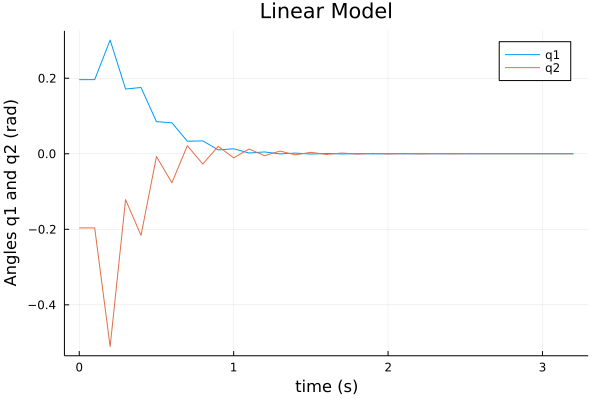
\includegraphics[width=0.50\columnwidth]{graphics/Chap09/q1q2LinearModelMPC.png}}%
}
\hspace{20pt }%
\subfloat[]{%
    \label{fig:LiDARmap}%
	\centering
	\setlength{\fboxsep}{0pt}%
\setlength{\fboxrule}{3pt}%
\fbox{
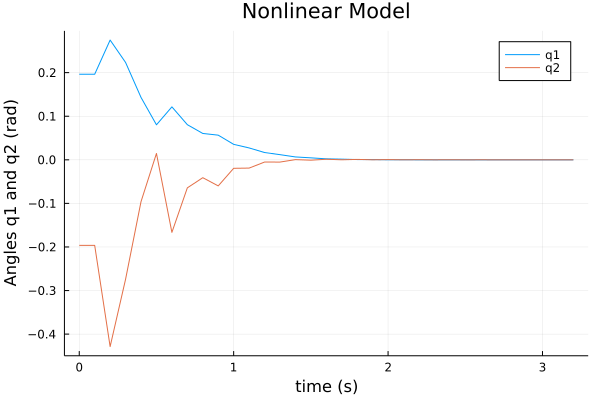
\includegraphics[width=0.50\columnwidth]{graphics/Chap09/q1q2NonlinearModelMPC.png}}%
}
\hspace{20pt }%
\subfloat[]{%
     
	\centering
		\setlength{\fboxsep}{0pt}%
\setlength{\fboxrule}{3pt}%
	\fbox{
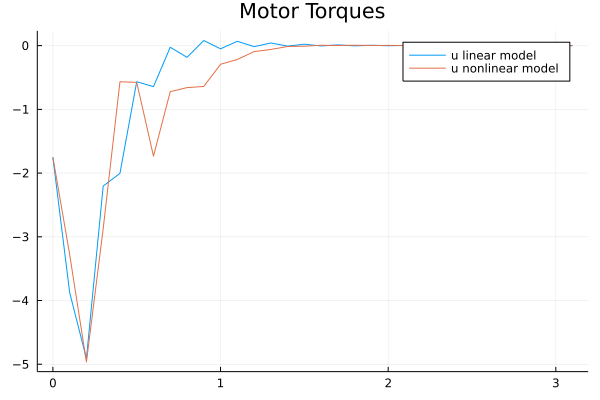
\includegraphics[width=0.50\columnwidth]{graphics/Chap09/torquesLinearNonlinearMPC.png}}%
}


\caption[]{Traces for the double inverted pendulum under MPC. The top plot is MPC applied to the linear model, where $q_1$ and $q_2$ converging to zero mean that they are going to the upright equilibrium. It is great but not surprising that it works. The middle plot is MPC applied to the nonlinear model, when the control is computed on the basis of a linear approximation. This is what is done on many real robots. It is awesome that this works! The bottom plot compares the torque commands for the motors in the two cases. They are remarkably similar. Larger initial deviations from the upright equilibrium can result in failure.}
    \label{fig:SnapShotFallingPendulum02}
\end{figure}

% \begin{lstlisting}[language=Julia,style=mystyle]

% \end{lstlisting}
% \textbf{Output} 
% \begin{verbatim}

% \end{verbatim}

% \begin{lstlisting}[language=Julia,style=mystyle]

% \end{lstlisting}
% \textbf{Output} 
% \begin{verbatim}

% \end{verbatim}

% \begin{lstlisting}[language=Julia,style=mystyle]

% \end{lstlisting}
% \textbf{Output} 
% \begin{verbatim}

% \end{verbatim}